\usetikzlibrary{decorations.markings}

\tikzset{->-/.style={decoration={
  markings,
  mark=at position #1 with {\arrow{>}}},postaction={decorate}}}
\tikzset{-<-/.style={decoration={
  markings,
  mark=at position #1 with {\arrow{<}}},postaction={decorate}}}


\newcommand{\IHmove}{\begin{tikzpicture}[ipe import, baseline, trim left]
  \node[ipe node, font=\normalsize, text=black]
     at (0, 64.001) {\begin{tikzpicture}[ipe import, baseline, trim left]
  \draw
    (16, 32)
     arc[start angle=90, end angle=270, radius=16];
  \draw
    (16, 32)
     .. controls (28, 32) and (28, 24) .. (36, 24);
  \draw
    (16, 0)
     .. controls (28, 0) and (28, 8) .. (36, 8);
  \draw
    (56, 0)
     arc[start angle=90, end angle=270, radius=-16];
  \draw[shift={(56, 0)}, scale=-1]
    (0, 0)
     .. controls (12, 0) and (12, -8) .. (20, -8);
  \draw[shift={(56, 32)}, scale=-1]
    (0, 0)
     .. controls (12, 0) and (12, 8) .. (20, 8);
  \draw
    (8, 16)
     .. controls (12, 12) and (20, 12) .. (24, 16);
  \draw
    (9.196, 14.9999)
     .. controls (13.732, 17) and (18.268, 17) .. (22.804, 14.9999);
  \draw
    (48, 16)
     .. controls (52, 12) and (60, 12) .. (64, 16);
  \draw
    (49.196, 15)
     .. controls (53.732, 17) and (58.268, 17) .. (62.804, 15);
\end{tikzpicture}
};
  \draw
    (140, 80.0006) circle[radius=12];
  \draw
    (188, 80.0006) circle[radius=12];
  \draw
    (152, 80.0006)
     -- (176, 80.0006);
  \draw
    (36, 16.0006) ellipse[x radius=36, y radius=16];
  \draw
    (24, 24.0006)
     .. controls (28, 20.0006) and (28, 12.0006) .. (24, 8.0006);
  \draw
    (24.7423, 23.1553)
     .. controls (12, 20.0006) and (12, 18.0006) .. (12, 16.0006)
     .. controls (12, 14.0006) and (12, 12.0006) .. (24.7423, 8.8459);
  \draw[shift={(48, 8.001)}, scale=-1]
    (0, 0)
     .. controls (4, -4) and (4, -12) .. (0, -16);
  \draw[shift={(47.258, 8.846)}, scale=-1]
    (0, 0)
     .. controls (-12.742, -3.155) and (-12.742, -5.155) .. (-12.742, -7.155)
     .. controls (-12.742, -9.155) and (-12.742, -11.155) .. (0, -14.31);
  \draw
    (164, 16) ellipse[x radius=36, y radius=16];
  \draw
    (164, 32.0006)
    -- (164, 0.0006);
    \node at (100, 80) {$=$};\node at (100, 15) {$=$};
    \draw[to-to] (37, 60)--(37, 38); \draw[to-to] (165, 60)--(165, 38);
    \node at (15, 50) {\scriptsize{IH move}};\node at (188, 50) {\scriptsize{IH move}};
\end{tikzpicture}}


\newcommand{\genusreduction}{\begin{tikzpicture}[ipe import, baseline, trim left]
  \draw[shift={(36.607, 39.125)}, xscale=0.9689, yscale=0.8868]
    (0, 0)
     .. controls (8, -12) and (24, -12) .. (32, 0);
  \draw
    (39.4122, 36.0015)
     .. controls (48, 44.002) and (56, 44.002) .. (64.5876, 36.0014);
  \draw
    (4, 56.002)
     .. controls (36, 72.002) and (44, 72.002) .. (52, 72.002)
     .. controls (60, 72.002) and (68, 72.002) .. (100, 56.002);
  \draw[shift={(4, 16.008)}, rotate=-0.0071]
    (0, 0)
     .. controls (32, -16) and (40, -16) .. (48, -16)
     .. controls (56, -16) and (64, -16) .. (96, 0);
  \draw[shift={(4.013, 16.002)}, xscale=0.334]
    (0, 0)
     .. controls (-12.0126, 8.0004) and (-12.0126, 14.0004) .. (-12.0126, 19.0004)
     .. controls (-12.0126, 24.0004) and (-12.0126, 28.0004) .. (-10.0126, 31.3337)
     .. controls (-8.0126, 34.667) and (-4.0126, 37.3337) .. (-2.0126, 38.667)
     .. controls (-0.0126, 40.0004) and (-0.0126, 40.0004) .. (-0.0126, 40.0004);
  \draw[shift={(3.987, 56.001)}, rotate=-179.9622, xscale=0.334]
    (0, 0)
     .. controls (-12.013, 8) and (-12.013, 14) .. (-12.013, 19)
     .. controls (-12.013, 24) and (-12.013, 28) .. (-10.013, 31.3333)
     .. controls (-8.013, 34.6667) and (-4.013, 37.3333) .. (-2.013, 38.6667)
     .. controls (-0.013, 40) and (-0.013, 40) .. (-0.013, 40);
  \draw[blue]
    (5.9177, 20.0016)
     .. controls (31.3059, 22.6685) and (45.3332, 26.4851) .. (47.9997, 31.4515);
  \draw[blue, dotted]
    (47.9997, 31.4515)
     .. controls (37.3332, 34.4851) and (21.3333, 34.6686) .. (0, 32.002);
  \draw[blue]
    (5.7414, 52.0014)
     .. controls (25.9138, 52.0018) and (39.9998, 48.4623) .. (47.9994, 41.3829);
  \draw[blue, dotted]
    (47.9994, 41.3829)
     .. controls (40, 40.002) and (12, 40.002) .. (0.2168, 44.0017);
  \draw[shift={(100.013, 16.002)}, xscale=0.334]
    (0, 0)
     .. controls (-12.013, 8) and (-12.013, 14) .. (-12.013, 19)
     .. controls (-12.013, 24) and (-12.013, 28) .. (-10.013, 31.3333)
     .. controls (-8.013, 34.6667) and (-4.013, 37.3333) .. (-2.013, 38.6667)
     .. controls (-0.013, 40) and (-0.013, 40) .. (-0.013, 40);
  \draw[shift={(99.987, 56.005)}, rotate=-179.9622, xscale=0.334]
    (0, 0)
     .. controls (-12.013, 8) and (-12.013, 14) .. (-12.013, 19)
     .. controls (-12.013, 24) and (-12.013, 28) .. (-10.013, 31.3333)
     .. controls (-8.013, 34.6667) and (-4.013, 37.3333) .. (-2.013, 38.6667)
     .. controls (-0.013, 40) and (-0.013, 40) .. (-0.013, 40);
  \draw[blue]
    (96.309, 28.0025)
     .. controls (80.103, 28.0021) and (68, 29.6209) .. (60.0001, 32.8587);
  \draw[blue, dotted]
    (60.0001, 32.8587)
     .. controls (76, 40.002) and (92, 40.002) .. (104, 40.002);
  \draw[green]
    (52, 36.002) ellipse[x radius=20, y radius=16];
  \draw[green]
    (36, 45.602)
     .. controls (36, 36.002) and (36, 34.002) .. (37, 31.002)
     .. controls (38, 28.002) and (40, 24.002) .. (44, 21.3377);
  \draw[green]
    (44, 50.6769)
     .. controls (44.0005, 39.5448) and (44.0005, 35.9756) .. (45.0004, 32.0899)
     .. controls (46.0003, 28.2042) and (48, 24.002) .. (52, 20.002);
  \draw[green]
    (52, 52.002)
     .. controls (52, 36.002) and (52, 28.002) .. (60, 21.3377);
  \draw[green]
    (60, 50.6662)
     .. controls (60, 36.002) and (64, 28.002) .. (67.9995, 26.4027);
  \draw
    (152, 56.002)
     .. controls (184, 72.002) and (192, 72.002) .. (200, 72.002)
     .. controls (208, 72.002) and (216, 72.002) .. (248, 56.002);
  \draw[shift={(152, 16.008)}, rotate=-0.0071]
    (0, 0)
     .. controls (32, -16) and (40, -16) .. (48, -16)
     .. controls (56, -16) and (64, -16) .. (96, 0);
  \draw[shift={(152.013, 16.002)}, xscale=0.334]
    (0, 0)
     .. controls (-12.013, 8) and (-12.013, 14) .. (-12.013, 19)
     .. controls (-12.013, 24) and (-12.013, 28) .. (-10.013, 31.3333)
     .. controls (-8.013, 34.6667) and (-4.013, 37.3333) .. (-2.013, 38.6667)
     .. controls (-0.013, 40) and (-0.013, 40) .. (-0.013, 40);
  \draw[shift={(151.987, 56.005)}, rotate=-179.9622, xscale=0.334]
    (0, 0)
     .. controls (-12.013, 8) and (-12.013, 14) .. (-12.013, 19)
     .. controls (-12.013, 24) and (-12.013, 28) .. (-10.013, 31.3333)
     .. controls (-8.013, 34.6667) and (-4.013, 37.3333) .. (-2.013, 38.6667)
     .. controls (-0.013, 40) and (-0.013, 40) .. (-0.013, 40);
  \draw[blue]
    (153.918, 20.002)
     .. controls (179.306, 22.6686) and (193.3333, 26.485) .. (196, 31.451);
  \draw[shift={(248.013, 16.002)}, xscale=0.334]
    (0, 0)
     .. controls (-12.013, 8) and (-12.013, 14) .. (-12.013, 19)
     .. controls (-12.013, 24) and (-12.013, 28) .. (-10.013, 31.3333)
     .. controls (-8.013, 34.6667) and (-4.013, 37.3333) .. (-2.013, 38.6667)
     .. controls (-0.013, 40) and (-0.013, 40) .. (-0.013, 40);
  \draw[shift={(247.987, 56.005)}, rotate=-179.9622, xscale=0.334]
    (0, 0)
     .. controls (-12.013, 8) and (-12.013, 14) .. (-12.013, 19)
     .. controls (-12.013, 24) and (-12.013, 28) .. (-10.013, 31.3333)
     .. controls (-8.013, 34.6667) and (-4.013, 37.3333) .. (-2.013, 38.6667)
     .. controls (-0.013, 40) and (-0.013, 40) .. (-0.013, 40);
  \draw[shift={(244.35, 28.55)}, rotate=1.2997, xscale=1.3305, yscale=0.8622, blue]
    (0, 0)
     .. controls (-16.206, 0) and (-28.309, 1.619) .. (-36.309, 4.857);
  \draw[blue]
    (153.7425, 52.0022)
     .. controls (184, 44.002) and (192, 36.002) .. (196.0009, 31.4507);
  \draw[blue, dotted]
    (148.2171, 44.0017)
     .. controls (169.4057, 46.6686) and (185.3333, 46.6686) .. (196, 44.002);
  \draw[blue, dotted]
    (148.0288, 32.0023)
     .. controls (169.3429, 32.0021) and (185.3334, 36.002) .. (196.0001, 44.002);
  \draw[blue, dotted]
    (251.9818, 40.0023)
     .. controls (227.9939, 42.6687) and (209.3335, 44.0021) .. (196.0005, 44.0022);
  \filldraw[fill=white]
    (196, 32.002) circle[radius=4.8];
  \filldraw[fill=white]
  (196, 44.002) circle[radius=4.8];
  \node at (196,44.5) {\tiny{$\varphi'$}};
  \node at (196,32) {\tiny{$\varphi$}};
  \node at (125, 36) {$=$};
\end{tikzpicture}
}

\newcommand{\stab}{\begin{tikzpicture}[ipe import, baseline, trim left]
\node at (75,30) {\footnotesize{$S$}};
  \draw
    (196, 8)
     .. controls (192, 8) and (192, 16) .. (191, 22)
     .. controls (190, 28) and (188, 32) .. (180, 32);
  \draw
    (132, 8)
     .. controls (136, 8) and (136, 16) .. (137, 22)
     .. controls (138, 28) and (140, 32) .. (148, 32);
  \draw
    (148, 32)
     -- (152, 32);
  \draw
    (176, 32)
     -- (180, 32);
  \draw
    (180, 8)
     .. controls (184, 12) and (184, 16) .. (183.3333, 18.6667)
     .. controls (182.6666, 21.3333) and (181.3333, 22.6667) .. (179.6666, 23.3333)
     .. controls (178, 24) and (176, 24) .. (176, 24);
  \draw
    (148, 8)
     .. controls (144, 12) and (144, 16) .. (145, 19)
     .. controls (146, 22) and (148, 24) .. (152, 24);
  \draw
    (152, 24)
     -- (164, 24);
  \draw
    (152, 32)
     -- (164, 32);
  \draw[red, dotted]
    (164, 32)
     .. controls (165.3333, 29.3334) and (165.3333, 26.6667) .. (164, 24);
  \draw[red]
    (164, 24)
     .. controls (162.6666, 26.6667) and (162.6666, 29.3334) .. (164, 32);
  \draw
    (164, 24)
     -- (176, 24);
  \draw
    (164, 32)
     -- (176, 32);
  \draw[dotted]
    (160, 8)
     arc[start angle=0, end angle=180, x radius=20, y radius=-8];
  \draw[dotted]
    (120, 8)
     .. controls (120, 13.3333) and (124, 16) .. (132, 16);
  \draw[dotted]
    (160, 8)
     .. controls (160, 13.3333) and (156, 16) .. (148, 16);
  \draw[dotted]
    (208, 8)
     arc[start angle=0, end angle=180, x radius=20, y radius=-8];
  \draw[dotted]
    (168, 8)
     .. controls (168, 13.3333) and (172, 16) .. (180, 16);
  \draw[dotted]
    (208, 8)
     .. controls (208, 13.3333) and (204, 16) .. (196, 16);
  \draw[blue]
    (123.551, 14.3364)
     .. controls (129.1836, 10.1121) and (129.6551, 6.2414) .. (124.9655, 2.7242);
  \draw[blue]
    (153.0309, 15.5471)
     .. controls (149.6769, 10.5157) and (149.931, 6.069) .. (153.7931, 2.2069);
  \draw[blue]
    (126.3949, 10)
     -- (126.0008, 12.1865);
  \draw[blue]
    (126.3949, 10)
     -- (126.0866, 11.7107);
  \draw[blue]
    (128, 12)
     .. controls (128, 12) and (126.0008, 12.1865) .. (126.0008, 12.1865);
  \draw[blue]
    (150, 10)
     -- (151.2308, 11.9998);
  \draw[blue]
    (152, 10)
     -- (151.2308, 11.9998);
  \draw[blue]
    (202, 7.9993)
     arc[start angle=0, end angle=180, x radius=14, y radius=-3.9993];
  \draw[shift={(174, 8)}, xscale=0.65, yscale=0.5, blue]
    (0, 0)
     .. controls (0, 5.3333) and (4, 8) .. (12, 8);
  \draw[shift={(202, 7.999)}, xscale=0.7, yscale=0.4999, blue]
    (0, 0)
     .. controls (0, 5.3333) and (-4, 8) .. (-12, 8);
  \draw[blue]
    (183.3958, 6.1132)
     -- (179.9998, 4.7172);
  \draw[shift={(182.673, 2.668)}, scale=0.7872, blue]
    (0, 0)
     .. controls (-2.264, 1.736) and (-3.396, 2.604) .. (-3.396, 2.604);
  \draw[dotted]
    (40, 8)
     arc[start angle=0, end angle=180, x radius=20, y radius=-8];
  \draw[dotted]
    (0, 8)
     .. controls (0, 13.3333) and (4, 16) .. (12, 16);
  \draw[dotted]
    (40, 8)
     .. controls (40, 13.3333) and (36, 16) .. (28, 16);
  \draw[dotted]
    (88, 8)
     arc[start angle=0, end angle=180, x radius=20, y radius=-8];
  \draw[dotted]
    (48, 8)
     .. controls (48, 13.3333) and (52, 16) .. (60, 16);
  \draw[dotted]
    (88, 8)
     .. controls (88, 13.3333) and (84, 16) .. (76, 16);
  \draw[blue]
    (3.551, 14.336)
     .. controls (9.1837, 10.112) and (9.6553, 6.2413) .. (4.966, 2.724);
  \draw[blue]
    (33.031, 15.547)
     .. controls (29.677, 10.5157) and (29.931, 6.069) .. (33.793, 2.207);
  \draw[blue]
    (6.395, 10)
     -- (6.001, 12.187);
  \draw[blue]
    (6.395, 10)
     -- (6.087, 11.711);
  \draw[blue]
    (8, 12)
     .. controls (8, 12) and (6.001, 12.187) .. (6.001, 12.187);
  \draw[blue]
    (30, 10)
     -- (31.231, 12);
  \draw[blue]
    (32, 10)
     -- (31.231, 12);
  \draw[blue]
    (82, 8)
     arc[start angle=0, end angle=180, x radius=14, y radius=-3.9993];
  \draw[shift={(54, 8)}, xscale=0.65, yscale=0.5, blue]
    (0, 0)
     .. controls (0, 5.3333) and (4, 8) .. (12, 8);
  \draw[shift={(82, 8)}, xscale=0.7, yscale=0.4999, blue]
    (0, 0)
     .. controls (0, 5.3333) and (-4, 8) .. (-12, 8);
  \draw[green]
    (20, 8)
     .. controls (20, 24) and (24, 28) .. (28, 28);
  \draw[green]
    (68, 8)
     .. controls (68, 24) and (64, 28) .. (60, 28);
  \draw[green]
    (28, 28)
     -- (60, 28);
  \draw[dotted]
    (12, 16)
     -- (16, 16);
  \draw[dotted]
    (24, 16)
     -- (28, 16);
  \draw[dotted]
    (60, 16)
     -- (64, 16);
  \draw[dotted]
    (72, 16)
     -- (76, 16);
  \pic[green]
     at (20, 8) {ipe disk};
  \pic[green]
     at (68, 8) {ipe disk};
  \draw[blue]
    (64, 6)
     -- (60.604, 4.604);
  \draw[shift={(63.277, 2.554)}, scale=0.7872, blue]
    (0, 0)
     .. controls (-2.264, 1.736) and (-3.396, 2.604) .. (-3.396, 2.604);
\end{tikzpicture}
}

\newcommand{\StabAndAfter}{\begin{tikzpicture}[ipe import, baseline, trim left]
  \draw
    (52.287, 0.1462)
     arc[start angle=-88.9742, end angle=91.0387, radius=16];
  \draw[shift={(51.714, 32.14)}, rotate=-178.9613]
    (0, 0)
     .. controls (8.0072, 0) and (8.0072, 4) .. (16.0072, 4);
  \draw[shift={(52.295, 0.145)}, rotate=-178.9613]
    (0, 0)
     .. controls (8.008, 0) and (8.008, -4) .. (16.008, -4);
  \draw[shift={(4.217, 3.854)}, rotate=-178.9613]
    (0, 0)
     .. controls (-2.6667, -8) and (-2.6667, -16) .. (0, -24);
  \draw[shift={(4.217, 3.854)}, rotate=-178.9613]
    (0, 0)
     .. controls (2.6667, -8) and (2.6667, -16) .. (0, -24);
  \draw
    (44.001, 17.6122)
     .. controls (48.001, 13.6122) and (56.001, 13.6122) .. (60.001, 17.6122);
  \draw
    (46.001, 16.1062)
     .. controls (50.001, 18.4435) and (54.001, 18.4435) .. (58.001, 16.1062);
  \draw
    (35.7818, 27.8492)
     -- (3.7818, 27.8492);
  \draw
    (4.2168, 3.8532)
     -- (36.2168, 3.8522);
  \draw[blue]
    (4.9708, 23.8482)
     .. controls (35.7818, 23.8492) and (43.7818, 19.8492) .. (46.0008, 16.1062);
  \draw[blue, dotted]
    (3.0298, 7.8492)
     .. controls (35.7818, 7.8492) and (43.7818, 11.8492) .. (46.0008, 16.1062);
  \draw[green]
    (51.7818, 15.8492) circle[radius=12];
  \draw[red]
    (58.0008, 16.1062)
     .. controls (59.7818, 19.8492) and (67.7818, 19.8492) .. (67.9978, 15.8492);
  \draw[red, dotted]
    (58.0018, 16.1072)
     .. controls (59.7818, 11.8492) and (67.7818, 11.8492) .. (67.9978, 15.8492);
  \draw
    (164.287, 0.1462)
     arc[start angle=-88.9742, end angle=91.0387, radius=16];
  \draw[shift={(163.714, 32.14)}, rotate=-178.9613]
    (0, 0)
     .. controls (8.0072, 0) and (8.0072, 4) .. (16.0072, 4);
  \draw[shift={(164.295, 0.145)}, rotate=-178.9613]
    (0, 0)
     .. controls (8.008, 0) and (8.008, -4) .. (16.008, -4);
  \draw[shift={(116.217, 3.854)}, rotate=-178.9613]
    (0, 0)
     .. controls (-2.6667, -8) and (-2.6667, -16) .. (0, -24);
  \draw[shift={(116.217, 3.854)}, rotate=-178.9613]
    (0, 0)
     .. controls (2.6667, -8) and (2.6667, -16) .. (0, -24);
  \draw
    (147.7818, 27.8492)
     -- (115.7818, 27.8492);
  \draw
    (116.2168, 3.8532)
     -- (148.2168, 3.8522);
  \draw[blue]
    (116.9708, 23.8492)
     .. controls (171.7818, 23.8492) and (179.7818, 19.8492) .. (179.7818, 15.8492);
  \draw[blue, dotted]
    (115.0298, 7.8482)
     .. controls (171.7818, 7.8492) and (179.7818, 11.8492) .. (179.7818, 15.8492);
  \draw[blue]
    (31.7818, 23.8492)
     -- (35.7813, 21.4812);
  \draw[blue]
    (35.7813, 21.4812)
     -- (31.7818, 19.8492);
  \draw[blue]
    (163.7818, 23.8492)
     -- (167.7818, 21.5352);
  \draw[blue]
    (163.7818, 19.8492)
     -- (167.7818, 21.5352);
  \node at (90,15) {$\longrightarrow$};
\end{tikzpicture}
}

\newcommand{\Slide}{\begin{tikzpicture}[ipe import, baseline, trim left]
  \draw[blue, dotted]
    (152, 128)
     arc[start angle=-90, end angle=90, x radius=16, y radius=-16];
  \draw[shift={(140, 100)}, xscale=1.5, dotted]
    (0, 0) rectangle (-16, 24);
  \draw[blue]
    (120, 144)
     -- (120, 128);
  \draw[blue]
    (120, 128)
     -- (128, 120);
  \draw[blue]
    (128, 120)
     -- (136, 128);
  \draw[shift={(128, 120)}, yscale=2, blue]
    (0, 0)
     -- (0, -8);
  \draw[blue]
    (128, 104)
     -- (120, 96);
  \draw[blue]
    (128, 104)
     -- (136, 96);
  \draw[shift={(120, 96)}, yscale=0.8, blue]
    (0, 0)
     -- (0, -20);
  \pic[blue]
     at (128, 120) {ipe disk};
  \pic[blue]
     at (128, 104) {ipe disk};
  \draw[blue]
    (136, 128)
     -- (152, 128);
  \draw[blue]
    (136, 96)
     -- (152, 96);
  \draw[blue, dotted]
    (40, 48)
     arc[start angle=-90, end angle=90, x radius=16, y radius=-16];
  \draw[blue]
    (8, 64)
     -- (8, 48);
  \draw[blue]
    (8, 48)
     -- (16, 40);
  \draw[blue]
    (16, 40)
     -- (24, 48);
  \draw[shift={(16, 40)}, yscale=2, blue]
    (0, 0)
     -- (0, -8);
  \draw[blue]
    (16, 24)
     -- (8, 16);
  \draw[blue]
    (16, 24)
     -- (24, 16);
  \draw[shift={(8, 16)}, yscale=0.8, blue]
    (0, 0)
     -- (0, -20);
  \pic[blue]
     at (16, 40) {ipe disk};
  \pic[blue]
     at (16, 24) {ipe disk};
  \draw[blue]
    (24, 48)
     -- (40, 48);
  \draw[blue]
    (24, 16)
     -- (40, 16);
  \draw[dotted]
    (12, 40)
     .. controls (12, 48) and (20, 52) .. (28, 52);
  \draw[dotted]
    (12, 40)
     .. controls (12, 36) and (14, 36) .. (15.6667, 36)
     .. controls (17.3333, 36) and (18.6667, 36) .. (19.3333, 36.6667)
     .. controls (20, 37.3333) and (20, 38.6667) .. (21, 40.3333)
     .. controls (22, 42) and (24, 44) .. (28, 44);
  \draw[dotted]
    (28, 44)
     -- (40, 44);
  \draw[dotted]
    (28, 52)
     -- (40, 52);
  \draw[dotted]
    (12, 24)
     .. controls (12, 28) and (14, 28) .. (15.6667, 28)
     .. controls (17.3333, 28) and (18.6667, 28) .. (19.3333, 27.3333)
     .. controls (20, 26.6667) and (20, 25.3333) .. (21, 23.6667)
     .. controls (22, 22) and (24, 20) .. (28, 20);
  \draw[dotted]
    (28, 20)
     -- (40, 20);
  \draw[dotted]
    (12, 24)
     .. controls (12, 16) and (20, 12) .. (28, 12);
  \draw[dotted]
    (28, 12)
     -- (40, 12);
  \draw[dotted]
    (40, 44)
     arc[start angle=-90, end angle=90, x radius=12, y radius=-12];
  \draw[dotted]
    (40, 52)
     arc[start angle=-90, end angle=90, x radius=20, y radius=-20];
  \draw[red, dotted]
    (152, 48)
     arc[start angle=-90, end angle=90, x radius=16, y radius=-16];
  \draw[blue]
    (120, 64)
     -- (120, 48);
  \draw[shift={(120, 16)}, yscale=0.8, blue]
    (0, 0)
     -- (0, -20);
  \draw[dotted]
    (124, 40)
     .. controls (124, 48) and (132, 52) .. (140, 52);
  \draw[dotted]
    (124, 40)
     .. controls (124, 36) and (126, 36) .. (127.6667, 36)
     .. controls (129.3333, 36) and (130.6667, 36) .. (131.3333, 36.6667)
     .. controls (132, 37.3333) and (132, 38.6667) .. (133, 40.3333)
     .. controls (134, 42) and (136, 44) .. (140, 44);
  \draw[dotted]
    (140, 44)
     -- (152, 44);
  \draw[dotted]
    (140, 52)
     -- (152, 52);
  \draw[dotted]
    (124, 24)
     .. controls (124, 28) and (126, 28) .. (127.6667, 28)
     .. controls (129.3333, 28) and (130.6667, 28) .. (131.3333, 27.3333)
     .. controls (132, 26.6667) and (132, 25.3333) .. (133, 23.6667)
     .. controls (134, 22) and (136, 20) .. (140, 20);
  \draw[dotted]
    (140, 20)
     -- (152, 20);
  \draw[dotted]
    (124, 24)
     .. controls (124, 16) and (132, 12) .. (140, 12);
  \draw[dotted]
    (140, 12)
     -- (152, 12);
  \draw[dotted]
    (152, 44)
     arc[start angle=-90, end angle=90, x radius=12, y radius=-12];
  \draw[dotted]
    (152, 52)
     arc[start angle=-90, end angle=90, x radius=20, y radius=-20];
  \draw[blue]
    (120, 48)
     -- (120, 16);
  \draw[red]
    (152, 48)
     .. controls (136, 48) and (128, 44) .. (128, 40);
  \draw[red]
    (152, 16)
     .. controls (132, 16) and (128, 20) .. (128, 24);
  \draw[red]
    (128, 24)
     -- (128, 40);
  \draw[red, dotted]
    (40, 128)
     arc[start angle=-90, end angle=90, x radius=16, y radius=-16];
  \draw[blue]
    (8, 144)
     -- (8, 128);
  \draw[shift={(8, 96)}, yscale=0.8, blue]
    (0, 0)
     -- (0, -20);
  \draw[blue]
    (8, 128)
     -- (8, 96);
  \draw[red]
    (40, 128)
     .. controls (24, 128) and (16, 124) .. (16, 120);
  \draw[red]
    (40, 96)
     .. controls (20, 96) and (16, 100) .. (16, 104);
  \draw[red]
    (16, 104)
     -- (16, 120);
  \draw[dotted]
    (24, 104) rectangle (0, 120);
  \draw[blue]
    (6, 132)
     -- (8, 128)
     -- (10, 132);
  \draw[blue]
    (6, 56)
     -- (8, 52)
     -- (10, 56);
  \draw[blue]
    (118, 56)
     -- (120, 52)
     -- (122, 56);
  \draw[blue]
    (118, 140)
     -- (120, 136)
     -- (122, 140);
\node at (85,30) {$=$};
\node at (-20,30) {$= \sum $};
\node at (85,110) {$= \sum $};
\node at (32, 110) {\scriptsize{$D_1$}};
\node at (148, 110) {\scriptsize{$D_1$}};
\node at (50, 60) {\scriptsize{$D_2$}};
\node at (160, 60) {\scriptsize{$D_2$}};
\end{tikzpicture}
}


\newcommand{\PipeSlide}{\begin{tikzpicture}[ipe import, baseline, trim left]
  \draw[shift={(0, 80)}, yscale=0.75]
    (0, 0)
     -- (0, -64);
  \draw
    (16, 80)
     -- (16, 32);
  \draw[red, dotted]
    (0, 56)
     arc[start angle=180, end angle=360, x radius=8, y radius=-4];
  \draw[red]
    (16, 56)
     arc[start angle=0, end angle=180, x radius=8, y radius=-4];
  \draw[blue]
    (48, 80)
     -- (16, 0);
  \draw[blue]
    (38, 62)
     -- (41.6, 64);
  \draw[blue]
    (42, 60)
     -- (41.6, 64);
  \draw[shift={(96, 80)}, yscale=0.75]
    (0, 0)
     -- (0, -64);
  \draw
    (112, 80)
     -- (112, 32);
  \draw[red, dotted]
    (96, 56)
     arc[start angle=180, end angle=360, x radius=8, y radius=-4];
  \draw[red]
    (112, 56)
     arc[start angle=0, end angle=180, x radius=8, y radius=-4];
  \draw[blue]
    (134, 62)
     -- (137.6, 64);
  \draw[blue]
    (138, 60)
     -- (137.6, 64);
  \draw[blue]
    (112, 44)
     .. controls (112, 40) and (108, 40) .. (106, 40)
     .. controls (104, 40) and (104, 40) .. (104, 36);
  \draw[blue]
    (96, 44)
     .. controls (96, 40) and (98, 40) .. (99, 40)
     .. controls (100, 40) and (100, 40) .. (100, 36);
  \draw[shift={(104, 36)}, yscale=0.75, blue]
    (0, 0)
     .. controls (0, -16) and (0, -16) .. (4, -16);
  \draw[shift={(100, 36)}, yscale=0.8, blue]
    (0, 0)
     .. controls (0, -20) and (0, -20) .. (8, -20);
  \draw[blue]
    (108, 24)
     .. controls (117.0667, 24) and (121.8667, 24.6667) .. (122.4, 26);
  \draw[blue]
    (108, 20)
     .. controls (116, 20) and (119.7333, 19.3333) .. (119.2, 18);
  \draw[blue]
    (112, 0)
     -- (119.2, 18);
  \draw[blue]
    (122.4, 26)
     -- (144, 80);
  \draw[blue, dotted]
    (96, 44)
     .. controls (96, 46.6667) and (98.6667, 48) .. (104, 48);
  \draw[blue, dotted]
    (112, 44)
     .. controls (112, 46.6667) and (109.3333, 48) .. (104, 48);
  \draw[shift={(208, 80)}, yscale=0.75]
    (0, 0)
     -- (0, -64);
  \draw
    (224, 80)
     -- (224, 32);
  \draw[red, dotted]
    (208, 56)
     arc[start angle=180, end angle=360, x radius=8, y radius=-4];
  \draw[red]
    (224, 56)
     arc[start angle=0, end angle=180, x radius=8, y radius=-4];
  \draw[blue]
    (246, 62)
     -- (249.6, 64);
  \draw[blue]
    (250, 60)
     -- (249.6, 64);
  \draw[blue]
    (220, 20)
     .. controls (228, 20) and (231.7333, 19.3333) .. (231.2, 18);
  \draw[blue]
    (224, 0)
     -- (231.2, 18);
  \draw[blue]
    (244.801, 52.002)
     .. controls (243.7337, 49.334) and (238.1333, 48) .. (228, 48);
  \draw[blue]
    (204, 48)
     .. controls (192, 48) and (192, 40) .. (192, 36);
  \draw[blue]
    (192, 36)
     .. controls (192, 28) and (192, 20) .. (204, 20);
  \draw[blue]
    (204, 20)
     -- (220, 20);
  \draw[blue]
    (244.801, 52.002)
     -- (256, 80);
\node at (160, 35) {$\longrightarrow$};
\node at (60, 35) {$\longrightarrow$};
\end{tikzpicture}
}


\newcommand{\KirbyZero}{\raise -4.5em
\hbox{
\begin{tikzpicture}
\begin{knot}
\begin{scope}
  \draw (-1,0.3) ellipse (0.3 and 0.1);
  \draw (-1.3,0.3)--(-1.3,-1.2); \draw (-0.7,0.3)--(-0.7,-1.2);
  \draw[blue, ->-=0.7] (-1, 0.2)--(-1,-1.2);
\end{scope}
  \draw (-2,-1) arc (180:360:1 and 0.4);
  \draw (-2,-1) arc (180:120:1 and 0.4);
  \draw (0,-1) arc (0:60:1 and 0.4);
  \draw (-2.4,-1) arc (180:360:1.4 and 0.8);
  \draw (-2.4,-1) arc (180:110:1.4 and 0.8);
  \draw (0.4,-1) arc (0:70:1.4 and 0.8);
  \draw[red] (-2.2,-1) arc (180:360:1.2 and 0.6);
  \draw[red] (-2.2,-1) arc (180:115:1.2 and 0.6);
  \draw[red] (0.2,-1) arc (0:65:1.2 and 0.6);
\begin{scope}
  \draw[dotted] (-1.3,-2.8) arc (180:0:0.3 and 0.1);
  \draw (-1.3,-2.8) arc (180:360:0.3 and 0.1);
  \draw (-1.3,-2)--(-1.3,-2.8); \draw (-0.7,-2)--(-0.7,-2.8);
  \draw[blue] (-1, -2)--(-1,-2.9);
\end{scope}
\begin{scope}[shift={(2.4,0)}]
  \draw (-2.4, -1) arc (180:0:0.2 and 0.1);
  \draw[dotted] (-2.4, -1) arc (180:360:0.2 and 0.1);
\end{scope}
\end{knot}
\end{tikzpicture}}
\quad \longrightarrow \quad
\raise -4.5em
\hbox{
\begin{tikzpicture}
\begin{knot}
  \draw (-1,0.3) ellipse (0.3 and 0.1);
  \draw (-1.3,0.3)--(-1.3,-0.7);
  \draw (-0.7,0.3)--(-0.7,-1.3);
  \draw[blue, ->-=0.7] (-1, 0.2)--(-1,-1.2);
  \strand (-1.3,-0.7) to[out=down,in=right] (-1.85,-0.9);
  \draw (-1.85,-0.9) arc (180:145:1.85 and 0.4);
  \strand (-1.85,-1.1) to[out=right,in=up] (-1.3,-1.3);
  \draw (-1.85,-1.1) arc (180:270:0.85 and 0.3);
  \draw[red] (-1.6,-0.9) arc (90:270:0.05 and 0.1);
  \draw[dotted, red] (-1.6,-0.9) arc (90:-90:0.05 and 0.1);
\begin{scope}
  \draw (0,-1) arc (0:60:1 and 0.4);
  \draw (0,-1) arc (0:-90:1 and 0.4); 
  \draw (-2.4,-1) arc (180:360:1.4 and 0.8);
  \draw (-2.4,-1) arc (180:110:1.4 and 0.8);
  \draw (0.4,-1) arc (0:70:1.4 and 0.8);
  \draw[red] (-2.2,-1) arc (180:360:1.2 and 0.6);
  \draw[red] (-2.2,-1) arc (180:115:1.2 and 0.6);
  \draw[red] (0.2,-1) arc (0:65:1.2 and 0.6);
\end{scope}
\begin{scope}
  \draw[dotted] (-1.3,-2.8) arc (180:0:0.3 and 0.1);
  \draw (-1.3,-2.8) arc (180:360:0.3 and 0.1);
  \draw (-1.3,-2)--(-1.3,-2.8); \draw (-0.7,-2)--(-0.7,-2.8);
  \draw[blue] (-1, -2)--(-1,-2.9);
\end{scope}
\begin{scope}[shift={(2.4,0)}]
  \draw (-2.4, -1) arc (180:0:0.2 and 0.1);
  \draw[dotted] (-2.4, -1) arc (180:360:0.2 and 0.1);
\end{scope}
\end{knot}
\end{tikzpicture}}
\quad \longrightarrow \quad
\raise -4.5em
\hbox{
\begin{tikzpicture}
\begin{knot}
  \draw (-1,0.3) ellipse (0.3 and 0.1);
  \draw (-1.3,0.3)--(-1.3,-0.7);
  \draw (-0.7,0.3)--(-0.7,-1.2);
  \draw[blue, ->-=0.7] (-1, 0.2)--(-1,-1.2);
  \strand (-1.3,-0.7) to[out=down,in=right] (-1.85,-0.9);
  \draw (-1.85,-0.9) arc (180:145:1.85 and 0.4);
  \strand (-1.85,-1.1) to[out=right,in=up] (-1.3,-1.3);  
  \draw (-1.85,-1.1) arc (180:270:0.85 and 0.3);
  \draw[green] (-1.75, -0.87) arc (180:150:1.75 and 0.25);
  \strand[green] (-1.75, -0.87)--(-1.5,-0.85);
  \draw[green] (-1.78, -1.15) arc (180:270:0.78 and 0.2);
  \strand[green] (-1.78,-1.15) to[out=right,in=left] (-1, -1.25);
  \draw[green] (-1,-1.25) arc (-90:50:0.65 and 0.25);
  \draw[green] (-1, -1.35) arc (-90:55:0.8 and 0.35);
\begin{scope}
  \draw (0,-1) arc (0:60:1 and 0.4);
  \draw (0,-1) arc (0:-90:1 and 0.4); 
  \draw (-2.4,-1) arc (180:360:1.4 and 0.8);
  \draw (-2.4,-1) arc (180:110:1.4 and 0.8);
  \draw (0.4,-1) arc (0:70:1.4 and 0.8);
  \draw[red] (-2.2,-1) arc (180:360:1.2 and 0.6);
  \draw[red] (-2.2,-1) arc (180:115:1.2 and 0.6);
  \draw[red] (0.2,-1) arc (0:65:1.2 and 0.6);
\end{scope}
\begin{scope}
  \draw[dotted] (-1.3,-2.8) arc (180:0:0.3 and 0.1);
  \draw (-1.3,-2.8) arc (180:360:0.3 and 0.1);
  \draw (-1.3,-2)--(-1.3,-2.8); \draw (-0.7,-2)--(-0.7,-2.8);
  \draw[blue] (-1, -2)--(-1,-2.9);
\end{scope}
\begin{scope}[shift={(2.4,0)}]
  \draw (-2.4, -1) arc (180:0:0.2 and 0.1);
  \draw[dotted] (-2.4, -1) arc (180:360:0.2 and 0.1);
\end{scope}
\end{knot}
\node[fill, white, inner sep = 1pt] at (-1.32,-1.265) {};
\fill[white] (-1.32, -1.256) circle (1pt);
\begin{scope}[shift={(-1.7,-1.15)}, xscale=0.14, yscale=0.14]
  \draw[green] (0,0)--(1,-1);
\end{scope}
\begin{scope}[shift={(-1.4,-1.2)}, xscale=0.14, yscale=0.14]
  \draw[green] (0,0)--(1,-1);
\end{scope}
\begin{scope}[shift={(-1.1,-1.25)}, xscale=0.1, yscale=0.1]
  \draw[green] (0,0)--(1,-1);
\end{scope}
\begin{scope}[shift={(-0.8,-1.24)}, xscale=0.09, yscale=0.09]
  \draw[green] (0,0)--(1,-1);
\end{scope}
\begin{scope}[shift={(-0.5,-1.16)}, xscale=0.08, yscale=0.08]
  \draw[green] (0,0)--(1,-1);
\end{scope}
\begin{scope}[shift={(-1.66,-0.79)}, xscale=0.07, yscale=0.07]
  \draw[green] (0,0)--(1,-1);
\end{scope}
\draw[green] (-0.4,-0.9)--(-0.3,-0.83);
\draw[green] (-0.37,-1.05)--(-0.215,-1.06);
\end{tikzpicture}}
\quad \longrightarrow \quad D\cdot \sum 
\raise -4.5em
\hbox{
\begin{tikzpicture}
\begin{knot}
  \node (A) [draw] at (-1, -0.8) {\tiny{$\varphi$}};
  \node (B) [draw] at (-1, -1.8) {\tiny{$\varphi$}};
  \draw (-1,0.3) ellipse (0.3 and 0.1);
  \draw (-1.3,0.3)--(-1.3,-2.8); \draw (-0.7,0.3)--(-0.7,-2.8);
  \draw[blue, ->-=0.7] (-1, 0.2)--(A.north);
  \draw[blue] (B.south)--(-1,-2.9);
\begin{scope}
  \draw[dotted] (-1.3,-2.8) arc (180:0:0.3 and 0.1);
  \draw (-1.3,-2.8) arc (180:360:0.3 and 0.1);
\end{scope}
\begin{scope}[red, shift={(0,1.5)}]
  \draw[dotted] (-1.3,-2.8) arc (180:0:0.3 and 0.1);
  \draw (-1.3,-2.8) arc (180:360:0.3 and 0.1);
\end{scope}
\end{knot}
\end{tikzpicture}
}}


\newcommand{\KirbyOneFirstStep}{\raisebox{-4.6em}{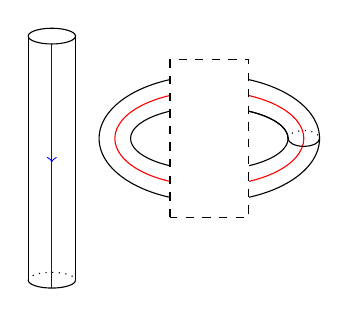
\begin{tikzpicture}
\begin{scope}[shift = {(-2,0)}]
  \draw (-1,0.3) ellipse (0.3 and 0.1);
  \draw (-1.3,0.3)--(-1.3,-2.8); \draw (-0.7,0.3)--(-0.7,-2.8);
  \draw[blue, ->-=0.5] (-1, 0.2)--(-1,-2.8);
  \draw[dotted] (-1.3,-2.8) arc (180:0:0.3 and 0.1);
  \draw (-1.3,-2.8) arc (180:360:0.3 and 0.1);
  \draw[blue] (-1, -2)--(-1,-2.9);
\end{scope}
  \draw (-2,-1) arc (180:540:1 and 0.4);
  \draw (0,-1) arc (0:60:1 and 0.4);
  \draw (-2.4,-1) arc (180:540:1.4 and 0.8);
  \draw[red] (-2.2,-1) arc (180:540:1.2 and 0.6);
\begin{scope}[shift={(2.4,0)}]
  \draw[dotted] (-2.4, -1) arc (180:0:0.2 and 0.1);
  \draw (-2.4, -1) arc (180:360:0.2 and 0.1);
\end{scope}
\begin{scope}[shift={(-1.5,-2)}]
  \draw[dashed, fill=white] (0,0) rectangle (1,2);
\end{scope}
\end{tikzpicture}}
\quad\longrightarrow\quad
\raisebox{-4.6em}{\begin{tikzpicture}
\begin{scope}[shift = {(-2,0)}]
  \begin{knot}
  \draw (-1,0.3) ellipse (0.3 and 0.1);
  \draw (-1.3,0.3)--(-1.3,-2.8); \draw (-0.7,0.3)--(-0.7,-0.8);
  \draw (-0.7,-1.5)--(-0.7,-2.8);
  \draw[blue, ->-=0.5] (-1, 0.2)--(-1,-2.8);
  \draw[dotted] (-1.3,-2.8) arc (180:0:0.3 and 0.1);
  \draw (-1.3,-2.8) arc (180:360:0.3 and 0.1);
  \draw[blue] (-1, -2)--(-1,-2.9);
  \strand (-0.7,-0.8) to [out=down, in=left] (-0.5,-1) to [out=right,in=down] (-0.3,-0.8);
  \strand (-0.7,-1.5) to [out=up,in=left] (-0.5,-1.3) to [out=right,in=up] (-0.3,-1.5);
  \draw[red] (-0.5,-1) arc (90:270:0.05 and 0.15);
  \draw[red, dotted] (-0.5,-1) arc (90:-90:0.05 and 0.15);
  \draw (-0.3,-0.8) arc (180:0:1.4 and 0.8);
  \draw (-0.3,-1.5) arc (180:360:1.4 and 0.8);
  \draw (2.5,-0.8)--(2.5,-1.5);
  \draw (2.1,-1) arc (0:180:1 and 0.4);
  \draw (2.1,-1.3) arc (0:-180:1 and 0.4);
  \draw (2.1,-1)--(2.1,-1.3);\draw(0.1,-1)--(0.1,-1.3);
\begin{scope}[red]
  \draw (-0.1,-0.9) arc (180:0:1.2 and 0.6);
  \draw (2.3,-1.4) arc (360:180:1.2 and 0.6);
  \draw (2.3,-1.4)--(2.3,-0.9);\draw (-0.1,-0.9)--(-0.1,-1.4);
\end{scope}
  \end{knot}
\end{scope}
\begin{scope}[shift={(2.5,-0.15)}]
  \draw[dotted] (-2.4, -1) arc (180:0:0.2 and 0.1);
  \draw (-2.4, -1) arc (180:360:0.2 and 0.1);
\end{scope}
\begin{scope}[shift={(-1.6,-2.4)}]
  \draw[dashed, fill=white] (0,0) rectangle (1.4,2.6);
\end{scope}
\end{tikzpicture}}
\quad\longrightarrow\quad
\raisebox{-4.6em}{\begin{tikzpicture}
\begin{scope}[shift = {(-2,0)}]
  \begin{knot}
  \draw (-1,0.3) ellipse (0.3 and 0.1);
  \draw (-1.3,0.3)--(-1.3,-2.8); \draw (-0.7,0.3)--(-0.7,-0.8);
  \draw (-0.7,-1.5)--(-0.7,-2.8);
  \draw[blue, ->-=0.5] (-1, 0.2)--(-1,-2.8);
  \draw[dotted] (-1.3,-2.8) arc (180:0:0.3 and 0.1);
  \draw (-1.3,-2.8) arc (180:360:0.3 and 0.1);
  \draw[blue] (-1, -2)--(-1,-2.9);
  \strand (-0.7,-0.8) to [out=down, in=left] (-0.5,-1) to [out=right,in=down] (-0.3,-0.8);
  \strand (-0.7,-1.5) to [out=up,in=left] (-0.5,-1.3) to [out=right,in=up] (-0.3,-1.5);
  \draw (-0.3,-0.8) arc (180:0:1.4 and 0.8);
  \draw (-0.3,-1.5) arc (180:360:1.4 and 0.8);
  \draw (2.5,-0.8)--(2.5,-1.5);
  \draw (2.1,-1) arc (0:180:1 and 0.4);
  \draw (2.1,-1.3) arc (0:-180:1 and 0.4);
  \draw (2.1,-1)--(2.1,-1.3);\draw(0.1,-1)--(0.1,-1.3);
\begin{scope}[red]
  \draw (-0.1,-0.9) arc (180:0:1.2 and 0.6);
  \draw (2.3,-1.4) arc (360:180:1.2 and 0.6);
  \draw (2.3,-1.4)--(2.3,-0.9);\draw (-0.1,-0.9)--(-0.1,-1.4);
\end{scope}
  \end{knot}
\end{scope}
\begin{scope}[shift={(2.5,-0.15)}]
  \draw[dotted] (-2.4, -1) arc (180:0:0.2 and 0.1);
  \draw (-2.4, -1) arc (180:360:0.2 and 0.1);
\end{scope}
\begin{scope}[shift={(-1.6,-2.4)}]
  \draw[dashed, fill=white] (0,0) rectangle (1.4,2.6);
\end{scope}
\end{tikzpicture}}}

\newcommand{\KirbyOneSecondStep}{  D\sum \raisebox{-4.6em}{\begin{tikzpicture}
\begin{scope}[shift = {(-2,0)}]
  \begin{knot}
  \draw (-1,0.3) ellipse (0.3 and 0.1);
  \strand (-1.3,0.3) to (-1.3, -1) to[out=down,in=up] (-1.1, -1.2) to[out=down,in=up] (-1.3,-1.4) to (-1.3,-2.8);
  \draw (-0.7,0.3)--(-0.7,-0.8);
  \draw (-0.7,-1.5)--(-0.7,-2.8);
  \draw[blue, ->-=0.5] (-1, 0.2)--(-1,-0.8); \draw[blue] (-1,-1.5)--(-1,-2.8);
  \draw[dotted] (-1.3,-2.8) arc (180:0:0.3 and 0.1);
  \draw (-1.3,-2.8) arc (180:360:0.3 and 0.1);
  \draw[blue] (-1, -2)--(-1,-2.9);
  \strand (-0.7,-0.8) to [out=down, in=left] (-0.5,-1) to [out=right,in=down] (-0.3,-0.8);
  \strand (-0.7,-1.5) to [out=up,in=left] (-0.5,-1.3) to [out=right,in=up] (-0.3,-1.5);
  \draw (-0.3,-0.8) arc (180:0:1.4 and 0.8);
  \draw (-0.3,-1.5) arc (180:360:1.4 and 0.8);
  \draw (2.5,-0.8)--(2.5,-1.5);
  \draw (2.1,-1) arc (0:180:1 and 0.4);
  \draw (2.1,-1.3) arc (0:-180:1 and 0.4);
  \draw (2.1,-1)--(2.1,-1.3);\draw(0.1,-1)--(0.1,-1.3);
\begin{scope}[red]
  \draw (-0.1,-0.9) arc (180:0:1.2 and 0.6);
  \draw (2.3,-1.4) arc (360:180:1.2 and 0.6);
  \draw (2.3,-1.4)--(2.3,-0.9);\draw (-0.1,-0.9)--(-0.1,-1.4);
\end{scope}
\begin{scope}[blue]
  \draw (2.4,-0.8) arc (0:180:1.3 and 0.7);
  \draw (2.4,-1.5) arc (360:180:1.3 and 0.7);
  \draw (2.4,-1.5)--(2.4,-0.8);
  \draw (-0.5,-1.1) arc (270:180:0.5 and 0.3); \draw (-0.5,-1.1) arc (270:360:0.3);
  \draw (-0.5,-1.2) arc (90:180:0.5 and 0.3); \draw (-0.5,-1.2) arc (90:0:0.3);
\end{scope}
  \end{knot}
\end{scope}
\begin{scope}[shift={(2.5,-0.15)}]
  \draw[dotted] (-2.4, -1) arc (180:0:0.2 and 0.1);
  \draw (-2.4, -1) arc (180:360:0.2 and 0.1);
\end{scope}
\begin{scope}[shift={(-1.6,-2.4)}]
  \draw[dashed, fill=white] (0,0) rectangle (1.4,2.6);
\end{scope}
\end{tikzpicture}}
\quad\longrightarrow\quad
\raisebox{-4.6em}{
  \begin{tikzpicture}\begin{scope}[scale=0.65,xscale=-1]
  \begin{scope}[shift={(0,0.5)}]
    \begin{knot}
    \draw (-0.7,-0.8) arc (180:0:1.8 and 1.1);
    \draw (-1.3,-0.8) arc (180:0:2.4 and 1.7);  
    \draw[blue, -<-=0.2] (-1,-0.8) arc (180:0:2.1 and 1.4);
    \draw (3.5, -0.8) arc (180:360:0.2 and 0.1);
    \draw[blue] (3.2, -0.8) arc (180:360:0.5 and 0.3);
    \draw (2.9, -0.8) arc (180:360:0.8 and 0.5);
    \strand (-0.7,-0.8) to [out=down, in=left] (-0.5,-1) to [out=right,in=down] (-0.3,-0.8);
    \draw (-0.3,-0.8) arc (180:0:1.4 and 0.8);
    \draw[red] (-0.1,-0.9) arc (180:0:1.2 and 0.6);
    \draw (2.1,-1) arc (0:180:1 and 0.4);
    \draw (-1.3,-0.8)--(-1.3,-1.5);\draw[blue] (-1,-0.8)--(-1,-1.5); \draw[red] (-0.1,-0.9)--(-0.1,-1.5);\draw (0.1,-1)--(0.1,-1.5); \draw (2.1,-1)--(2.1,-1.5); \draw[red] (2.3,-0.9)--(2.3,-1.5); \draw (2.5,-0.8)--(2.5,-1.5);
    \draw (3.9,-0.8)--(3.9,1);\draw[blue] (4.2,-0.8)--(4.2,0.9);\draw (4.5,-0.8)--(4.5,1);
    \draw (4.2,1) ellipse (0.3 and 0.1);
    \end{knot}
  \end{scope}
  \begin{scope}[shift={(0,-2.5)}, yscale=-1]
    \begin{knot}
    \draw[dotted] (1.1,0.9) arc (90:270:0.15 and 0.3);\draw (1.1,0.9) arc (90:-90:0.15 and 0.3);
    \draw (-0.7,-0.8) arc (180:0:1.8 and 1.1);
    \draw (-1.3,-0.8) arc (180:0:2.4 and 1.7);  
    \draw[blue] (-1,-0.8) arc (180:0:2.1 and 1.4);
    \draw (3.5, -0.8) arc (180:360:0.2 and 0.1);
    \draw[blue] (3.2, -0.8) arc (180:360:0.5 and 0.3);
    \draw (2.9, -0.8) arc (180:360:0.8 and 0.5);
    \strand (-0.7,-0.8) to [out=down, in=left] (-0.5,-1) to [out=right,in=down] (-0.3,-0.8);
    \draw (-0.3,-0.8) arc (180:0:1.4 and 0.8);
    \draw[red] (-0.1,-0.9) arc (180:0:1.2 and 0.6);
    \draw (2.1,-1) arc (0:180:1 and 0.4);
    \draw (-1.3,-0.8)--(-1.3,-1.5);\draw[blue] (-1,-0.8)--(-1,-1.5); \draw[red] (-0.1,-0.9)--(-0.1,-1.5);\draw (0.1,-1)--(0.1,-1.5); \draw (2.1,-1)--(2.1,-1.5); \draw[red] (2.3,-0.9)--(2.3,-1.5); \draw (2.5,-0.8)--(2.5,-1.5);
    \draw (3.9,-0.8)--(3.9,1);\draw[blue] (4.2,-0.8)--(4.2,1.1);\draw (4.5,-0.8)--(4.5,1);
    \draw (3.9,1) arc (180:0:0.3 and 0.1); \draw[dotted] (3.9,1) arc (180:360:0.3 and 0.1);
    \end{knot}
  \end{scope}
\begin{scope}[shift={(4.5,0)}]
  \draw[dotted] (-2.4, -1) arc (180:0:0.2 and 0.1);
  \draw (-2.4, -1) arc (180:360:0.2 and 0.1);
\end{scope}
\begin{scope}[shift={(0.45,-2.4)}]
  \draw[dashed, fill=white] (0,-1.5) rectangle (1.3,4.1);
\end{scope}
\end{scope}
\end{tikzpicture}}
\quad\longrightarrow\quad
\raisebox{-4.6em}{
\begin{tikzpicture}\begin{scope}[scale=0.65,xscale=-1]
  \begin{scope}[shift={(0,0.5)}]
    \begin{knot}
    \draw (-0.7,-0.8) arc (180:0:1.8 and 1.1);
    \draw (-1.3,-0.8) arc (180:0:2.4 and 1.7);  
    \draw[blue, -<-=0.2] (-1,-0.8) arc (180:0:2.1 and 1.4);
    \draw (3.5, -0.8) arc (180:360:0.2 and 0.1);
    \draw[blue] (3.2, -0.8) arc (180:360:0.5 and 0.3);
    \draw (2.9, -0.8) arc (180:360:0.8 and 0.5);
    \strand (-0.7,-0.8) to [out=down, in=left] (-0.5,-1) to [out=right,in=down] (-0.3,-0.8);
    \draw (-0.3,-0.8) arc (180:0:1.4 and 0.8);
    \draw[red] (-0.1,-0.9) arc (180:0:1.2 and 0.6);
    \draw (2.1,-1) arc (0:180:1 and 0.4);
    \draw (-1.3,-0.8)--(-1.3,-1.5);\draw[blue] (-1,-0.8)--(-1,-1.5); \draw[red] (-0.1,-0.9)--(-0.1,-1.5);\draw (0.1,-1)--(0.1,-1.5); \draw (2.1,-1)--(2.1,-1.5); \draw[red] (2.3,-0.9)--(2.3,-1.5); \draw (2.5,-0.8)--(2.5,-1.5);
    \draw (3.9,-0.8)--(3.9,1);\draw[blue] (4.2,-0.8)--(4.2,0.9);\draw (4.5,-0.8)--(4.5,1);
    \draw (4.2,1) ellipse (0.3 and 0.1);
    \draw[red,dotted] (-0.5,-1) arc (90:180:0.1 and 0.5);\draw[red] (-0.5,-1) arc (90:0:0.1 and 0.5);
    \end{knot}
  \end{scope}
  \begin{scope}[shift={(0,-2.5)}, yscale=-1]
    \begin{knot}
    \draw[red,dotted] (-0.5,-1) arc (90:180:0.1 and 0.5);\draw[red] (-0.5,-1) arc (90:0:0.1 and 0.5); 
    \draw[dotted] (1.1,0.9) arc (90:270:0.15 and 0.3);\draw (1.1,0.9) arc (90:-90:0.15 and 0.3);
    \draw (-0.7,-0.8) arc (180:0:1.8 and 1.1);
    \draw (-1.3,-0.8) arc (180:0:2.4 and 1.7);  
    \draw[blue] (-1,-0.8) arc (180:0:2.1 and 1.4);
    \draw (3.5, -0.8) arc (180:360:0.2 and 0.1);
    \draw[blue] (3.2, -0.8) arc (180:360:0.5 and 0.3);
    \draw (2.9, -0.8) arc (180:360:0.8 and 0.5);
    \strand (-0.7,-0.8) to [out=down, in=left] (-0.5,-1) to [out=right,in=down] (-0.3,-0.8);
    \draw (-0.3,-0.8) arc (180:0:1.4 and 0.8);
    \draw[red] (-0.1,-0.9) arc (180:0:1.2 and 0.6);
    \draw (2.1,-1) arc (0:180:1 and 0.4);
    \draw (-1.3,-0.8)--(-1.3,-1.5);\draw[blue] (-1,-0.8)--(-1,-1.5); \draw[red] (-0.1,-0.9)--(-0.1,-1.5);\draw (0.1,-1)--(0.1,-1.5); \draw (2.1,-1)--(2.1,-1.5); \draw[red] (2.3,-0.9)--(2.3,-1.5); \draw (2.5,-0.8)--(2.5,-1.5);
    \draw (3.9,-0.8)--(3.9,1);\draw[blue] (4.2,-0.8)--(4.2,1.1);\draw (4.5,-0.8)--(4.5,1);
    \draw (3.9,1) arc (180:0:0.3 and 0.1); \draw[dotted] (3.9,1) arc (180:360:0.3 and 0.1);
    \end{knot}
  \end{scope}
\begin{scope}[shift={(4.5,0)}]
  \draw[dotted] (-2.4, -1) arc (180:0:0.2 and 0.1);
  \draw (-2.4, -1) arc (180:360:0.2 and 0.1);
\end{scope}
\begin{scope}[shift={(0.45,-2.4)}]
  \draw[dashed, fill=white] (0,-1.5) rectangle (1.3,4.1);
\end{scope}
\end{scope}
\end{tikzpicture}}}

\newcommand{\KirbyOneThirdStep}{\begin{tikzpicture}\begin{scope}[scale=0.65,xscale=-1]
  \begin{scope}[shift={(0,0.5)}]
    \begin{knot}
      \draw (-0.7,-0.8) arc (180:0:1.8 and 1.1);
    \draw (-0.7,-0.8)--(-0.7,-1.5);      \draw (-0.3,-0.8)--(-0.3,-1.5);
    \draw (-1.3,-0.8) arc (180:0:2.4 and 1.7);  
    \draw[blue, -<-=0.2] (-1,-0.8) arc (180:0:2.1 and 1.4);
    \draw (3.5, -0.8) arc (180:360:0.2 and 0.1);
    \draw[blue] (3.2, -0.8) arc (180:360:0.5 and 0.3);
    \draw (2.9, -0.8) arc (180:360:0.8 and 0.5);
    \draw (-0.3,-0.8) arc (180:0:1.4 and 0.8);
    \draw[red] (-0.1,-0.9) arc (180:0:1.2 and 0.6);
    \draw (2.1,-1) arc (0:180:1 and 0.4);
    \draw (-1.3,-0.8)--(-1.3,-1.5);\draw[blue] (-1,-0.8)--(-1,-1.5); \draw[red] (-0.1,-0.9)--(-0.1,-1.5);\draw (0.1,-1)--(0.1,-1.5); \draw (2.1,-1)--(2.1,-1.5); \draw[red] (2.3,-0.9)--(2.3,-1.5); \draw (2.5,-0.8)--(2.5,-1.5);
    \draw (3.9,-0.8)--(3.9,1);\draw[blue] (4.2,-0.8)--(4.2,0.9);\draw (4.5,-0.8)--(4.5,1);
    \draw (4.2,1) ellipse (0.3 and 0.1);
    \end{knot}
  \end{scope}
  \begin{scope}[shift={(0,-2.5)}, yscale=-1]
    \begin{knot}
    \draw (-0.7,-0.8)--(-0.7,-1.5);      \draw (-0.3,-0.8)--(-0.3,-1.5);
    \draw[dotted] (1.1,0.9) arc (90:270:0.15 and 0.3);\draw (1.1,0.9) arc (90:-90:0.15 and 0.3);
    \draw (-0.7,-0.8) arc (180:0:1.8 and 1.1);
    \draw (-1.3,-0.8) arc (180:0:2.4 and 1.7);  
    \draw[blue] (-1,-0.8) arc (180:0:2.1 and 1.4);
    \draw (3.5, -0.8) arc (180:360:0.2 and 0.1);
    \draw[blue] (3.2, -0.8) arc (180:360:0.5 and 0.3);
    \draw (2.9, -0.8) arc (180:360:0.8 and 0.5);
    \draw (-0.3,-0.8) arc (180:0:1.4 and 0.8);
    \draw[red] (-0.1,-0.9) arc (180:0:1.2 and 0.6);
    \draw (2.1,-1) arc (0:180:1 and 0.4);
    \draw (-1.3,-0.8)--(-1.3,-1.5);\draw[blue] (-1,-0.8)--(-1,-1.5); \draw[red] (-0.1,-0.9)--(-0.1,-1.5);\draw (0.1,-1)--(0.1,-1.5); \draw (2.1,-1)--(2.1,-1.5); \draw[red] (2.3,-0.9)--(2.3,-1.5); \draw (2.5,-0.8)--(2.5,-1.5);
    \draw (3.9,-0.8)--(3.9,1);\draw[blue] (4.2,-0.8)--(4.2,1.1);\draw (4.5,-0.8)--(4.5,1);
    \draw (3.9,1) arc (180:0:0.3 and 0.1); \draw[dotted] (3.9,1) arc (180:360:0.3 and 0.1);
    \end{knot}
  \end{scope}
\begin{scope}[shift={(4.5,0)}]
  \draw[dotted] (-2.4, -1) arc (180:0:0.2 and 0.1);
  \draw (-2.4, -1) arc (180:360:0.2 and 0.1);
\end{scope}
\begin{scope}[shift={(1.1,0)}]
  \draw[dotted] (-2.4, -1) arc (180:0:0.3 and 0.15);
  \draw (-2.4, -1) arc (180:360:0.3 and 0.15);
\end{scope}
\begin{scope}[shift={(0.45,-2.4)}]
  \draw[dashed, fill=white] (0,-1.5) rectangle (1.3,4.1);
\end{scope}
\end{scope}
\end{tikzpicture}}



\newcommand{\GenusOneCutOne}{\begin{tikzpicture}[ipe import, baseline, trim left,yscale=0.8]
\node at (80,105) {$\tiny{f}$};
\draw
    (80, 81.5058)
     .. controls (84, 77.5058) and (92, 77.5058) .. (96, 81.5058);
  \draw
    (82, 79.9998)
     .. controls (86, 82.3371) and (90, 82.3371) .. (94, 79.9998);
  \draw[blue]
    (80, 96)
     .. controls (80, 88) and (82.6667, 83.251) .. (88, 81.753);
  \draw[green]
    (64, 80)
     .. controls (64, 90.6667) and (69.3333, 96) .. (80, 96);
  \draw[green]
    (96, 96)
     .. controls (106.6667, 96) and (112, 90.6667) .. (112, 80);
  \draw[green]
    (80, 96)
     -- (96, 96);
  \draw[blue]
    (80, 96)
     -- (80, 104);
  \draw
    (72, 112) rectangle (88, 104);
  \draw[blue]
    (72, 108)
     .. controls (56, 108) and (48, 98.6667) .. (48, 80);
  \draw[blue]
    (104, 108)
     .. controls (120, 108) and (128, 98.6667) .. (128, 80);
  \draw[blue]
    (88, 108)
     -- (104, 108);
  \draw[shift={(80, 112)}, yscale=0.875, blue]
    (0, 0)
     -- (0, 32);
  \draw[green]
    (32, 80)
     .. controls (32, 112) and (42.6667, 128) .. (64, 128);
  \draw[green]
    (160, 80)
     .. controls (160, 112) and (149.3333, 128) .. (128, 128);
  \draw[green]
    (128, 128)
     .. controls (85.3333, 128) and (64, 128) .. (64, 128);
  \draw
    (72, 148) rectangle (88, 140);
  \draw[blue]
    (80, 152)
     .. controls (80, 157.3333) and (82.6667, 160) .. (88, 160);
  \draw[blue, dotted]
    (88, 160)
     .. controls (93.3333, 160) and (96, 157.3333) .. (96, 152);
  \draw[blue, dotted]
    (96, 152)
     -- (96, 96);
  \draw[blue, dotted]
    (88, 81.753)
     .. controls (93.3333, 83.251) and (96, 88) .. (96, 96);
  \draw[shift={(112, 80)}, scale=-1, green]
    (0, 0)
     .. controls (0, 10.6667) and (5.3333, 16) .. (16, 16);
  \draw[shift={(80, 64)}, scale=-1, green]
    (0, 0)
     .. controls (10.6667, 0) and (16, -5.3333) .. (16, -16);
  \draw[shift={(96, 64)}, scale=-1, green]
    (0, 0)
     -- (16, 0);
  \draw[shift={(104, 52)}, scale=-1, blue]
    (0, 0)
     .. controls (-16, 0) and (-24, -9.3333) .. (-24, -28);
  \draw[shift={(72, 52)}, scale=-1, blue]
    (0, 0)
     .. controls (16, 0) and (24, -9.3333) .. (24, -28);
  \draw[blue]
    (72, 52)
     -- (104, 52);
  \draw[shift={(160, 80)}, scale=-1, green]
    (0, 0)
     .. controls (0, 32) and (10.6667, 48) .. (32, 48);
  \draw[shift={(32, 80)}, scale=-1, green]
    (0, 0)
     .. controls (0, 32) and (-10.6667, 48) .. (-32, 48);
  \draw[shift={(64, 32)}, scale=-1, green]
    (0, 0)
     .. controls (-42.6667, 0) and (-64, 0) .. (-64, 0);
  \draw
    (0, 80)
     .. controls (0, 133.3333) and (16, 160) .. (48, 160);
  \draw
    (48, 160)
     -- (144, 160);
  \draw
    (144, 160)
     .. controls (176, 160) and (192, 133.3333) .. (192, 80);
  \draw[shift={(192, 80)}, scale=-1]
    (0, 0)
     .. controls (0, 53.3333) and (16, 80) .. (48, 80);
  \draw[shift={(144, 0)}, scale=-1]
    (0, 0)
     -- (96, 0);
  \draw[shift={(48, 0)}, scale=-1]
    (0, 0)
     .. controls (32, 0) and (48, -26.6667) .. (48, -80);
  \draw[blue]
    (80, 152)
     -- (80, 148);
  \draw[blue]
    (16, 80)
     .. controls (16, 136) and (44, 144) .. (48, 144);
  \draw[blue]
    (48, 144)
     -- (72, 144);
  \draw[blue]
    (16, 80)
     .. controls (16, 32) and (32, 16) .. (48, 16);
  \draw[blue]
    (48, 16)
     -- (144, 16);
  \draw[blue]
    (88, 144)
     -- (144, 144);
  \draw[blue]
    (144, 144)
     .. controls (160, 144) and (176, 136) .. (176, 80);
  \draw[blue]
    (176, 80)
     .. controls (176, 32) and (168, 16) .. (144, 16);
\end{tikzpicture}
}

\newcommand{\GenusOneCutTwo}{\begin{tikzpicture}[ipe import, baseline, trim left]
  \draw[shift={(56, 24)}, yscale=2]
    (0, 0) rectangle (16, -8);
  \draw
    (8, 24) rectangle (24, 8);
  \draw
    (24, 16)
     -- (56, 16);
  \draw[shift={(72, 16)}, xscale=0.6667]
    (0, 0)
     -- (48, 0);
  \draw
    (104, 24) rectangle (120, 8);
  \draw
    (152, 24) rectangle (168, 8);
  \draw
    (120, 16) rectangle (152, 16);
  \draw
    (64, 24)
     arc[start angle=0, end angle=90, radius=8];
  \draw
    (64, 8)
     arc[start angle=0, end angle=90, x radius=8, y radius=-8];
  \draw
    (0, 24)
     arc[start angle=180, end angle=270, x radius=8, y radius=-8];
  \draw
    (8, 0)
     arc[start angle=90, end angle=180, x radius=8, y radius=-8];
  \draw
    (0, 24)
     -- (0, 8);
  \draw
    (8, 0)
     -- (56, 0);
  \draw
    (8, 32)
     -- (56, 32);
  \draw
    (112, 24)
     arc[start angle=180, end angle=270, x radius=8, y radius=-8];
  \draw
    (112, 8)
     arc[start angle=180, end angle=270, radius=8];
  \draw
    (176, 24)
     arc[start angle=0, end angle=90, radius=8];
  \draw
    (168, 0)
     arc[start angle=-90, end angle=0, radius=8];
  \draw
    (120, 32)
     -- (168, 32);
  \draw
    (176, 24)
     -- (176, 8);
  \draw
    (120, 0)
     -- (168, 0);
\end{tikzpicture}
}

\newcommand{\GenusOneCutThree}{\begin{tikzpicture}[ipe import, baseline, trim left]
  \draw[shift={(64, 40)}, yscale=2]
    (0, 0) rectangle (16, -8);
  \draw
    (16, 40) rectangle (32, 24);
  \draw
    (32, 32)
     -- (64, 32);
  \draw
    (24.0474, 23.8122)
     arc[start angle=-179.6688, end angle=-89.6688, radius=8];
  \draw
    (23.9549, 39.8119)
     { [rotate=-179.6688] arc[start angle=0, end angle=90, x radius=8, y radius=-8] };
  \draw
    (88.0463, 24.1821)
     { [rotate=-179.6688] arc[start angle=180, end angle=270, x radius=8, y radius=-8] };
  \draw
    (79.9077, 48.1355)
     { [rotate=-179.6688] arc[start angle=90, end angle=180, x radius=8, y radius=-8] };
  \draw[shift={(88.046, 24.182)}, rotate=-179.6688]
    (0, 0)
     -- (0, -16);
  \draw[shift={(79.908, 48.135)}, rotate=-179.6688]
    (0, 0)
     -- (48, 0);
  \draw[shift={(80.093, 16.136)}, rotate=-179.6688]
    (0, 0)
     -- (48, 0);
  \draw[shift={(160, 40)}, yscale=2]
    (0, 0) rectangle (16, -8);
  \draw
    (112, 40) rectangle (128, 24);
  \draw
    (128, 32)
     -- (160, 32);
  \draw
    (168, 40)
     arc[start angle=0, end angle=90, radius=8];
  \draw
    (168, 24)
     arc[start angle=0, end angle=90, x radius=8, y radius=-8];
  \draw
    (104, 40)
     arc[start angle=180, end angle=270, x radius=8, y radius=-8];
  \draw
    (112, 16)
     arc[start angle=90, end angle=180, x radius=8, y radius=-8];
  \draw
    (104, 40)
     -- (104, 24);
  \draw
    (112, 16)
     -- (160, 16);
  \draw
    (112, 48)
     -- (160, 48);
  \draw
    (16, 32)
     arc[start angle=90, end angle=270, radius=16];
  \draw
    (176, 32)
     arc[start angle=-90, end angle=90, x radius=16, y radius=-16];
  \draw
    (16, 0)
     -- (176, 0);
\end{tikzpicture}
}

\newcommand{\GenusOneCutFour}{\begin{tikzpicture}[ipe import, baseline, trim left]
  \draw[shift={(56, 24)}, yscale=2]
    (0, 0) rectangle (16, -8);
  \draw
    (8, 24) rectangle (24, 8);
  \draw
    (24, 16)
     -- (56, 16);
  \draw
    (152, 24) rectangle (168, 8);
  \draw
    (200, 24) rectangle (216, 8);
  \draw
    (168, 16) rectangle (200, 16);
  \draw
    (64, 24)
     arc[start angle=0, end angle=90, radius=8];
  \draw
    (64, 8)
     arc[start angle=0, end angle=90, x radius=8, y radius=-8];
  \draw
    (0, 24)
     arc[start angle=180, end angle=270, x radius=8, y radius=-8];
  \draw
    (8, 0)
     arc[start angle=90, end angle=180, x radius=8, y radius=-8];
  \draw
    (0, 24)
     -- (0, 8);
  \draw
    (8, 0)
     -- (56, 0);
  \draw
    (8, 32)
     -- (56, 32);
  \draw
    (160, 24)
     arc[start angle=180, end angle=270, x radius=8, y radius=-8];
  \draw
    (160, 8)
     arc[start angle=180, end angle=270, radius=8];
  \draw
    (224, 24)
     arc[start angle=0, end angle=90, radius=8];
  \draw
    (216, 0)
     arc[start angle=-90, end angle=0, radius=8];
  \draw
    (168, 32)
     -- (216, 32);
  \draw
    (224, 24)
     -- (224, 8);
  \draw
    (168, 0)
     -- (216, 0);
  \draw
    (88, 24) rectangle (104, 8);
  \draw
    (120, 24) rectangle (136, 8);
  \draw
    (72, 16)
     -- (88, 16);
  \draw
    (136, 16)
     -- (152, 16);
\end{tikzpicture}
}